\documentclass[a4paper]{ctexart}
\usepackage{geometry}
\usepackage{listings}
\usepackage{hyperref}
\geometry{left=2cm,right=2cm,top=2.5cm,bottom=2.5cm}

\author{Chunwei Yan}
\title{关于作业1的一些想法}
\begin{document}
    \maketitle
%---content here----
\section{背景知识}
	\subsection{文件格式}
	
\paragraph{xml组织}
原始文件中,每一行为一个page,将一行展开,得到如下:
\begin{lstlisting}[language=XML]
 <title>AlgeriA</title>     
 <id>5</id>     
 <revision>       
	 <id>136471847</id>       
	 <timestamp>2007-06-06T23:05:07Z</timestamp>       
	 <contributor>         
	 <username>Cwschimpff</username>         
	 <id>4581842</id>       
	 </contributor>       
	 <comment>[[WP:AES|←]]Redirected page to [[Algeria]]</comment>       
	 <text xml:space="preserve">#REDIRECT [[Algeria]] {{R from CamelCase}}</text>     </revision>
\end{lstlisting}
\paragraph{ <title>AlgeriA</title>}
标记本page的title,\textbf{关键}
\paragraph{
 <id>5</id>     
}
在此文件中每个page有唯一的一个id号码,作为标识,其中,在wiki百科中,title和id均唯一。参照题目1的reference教程里面的图片;
\begin{center} 
    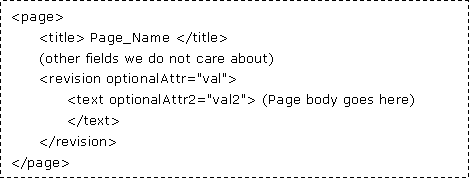
\includegraphics[width=0.7\textwidth]{image001.png}
\end{center}
可以认为id是可以忽略的。\textbf{可忽略}
\paragraph{
 <revision>...</revision>
}
里面应该只有<text>标签比较关键
\paragraph{ <text xml:space="preserve">...</text>}
包含文章的内容,包括wiki内部的链接在内\textbf{关键}

\subsection{wiki的内容格式}
wiki百科的网页内部,经常有关键词的相互引用.\\
可以查询下wiki百科的相关说明:
\url{http://en.wikipedia.org/wiki/Help:Wikilinks\#Wikilinks}
\paragraph{
	这里做一些摘录和解释
}
wikilink (or internal link) links a page to another page within English Wikipedia. Links are enclosed in doubled square brackets like this:\\

 [[abc]] is seen as "abc" in text and links to page "abc".\\

	 Use a vertical bar "|" (the "pipe" symbol – see Wikipedia:Piped link for how to type one) to create a link while labeling it with a different name on the original page. The first term inside the brackets is the link (the page you would be taken to), while anything you type after the vertical bar is what that link looks like on the original page. Here are some examples:\\
\begin{enumerate}
	\item $[[a|b]]$ is labeled "b" on this page but links to page "a".
	\item $[[a]]b$ gives ab. So does [[a|ab]]: ab. [[a|b]]c gives bc, just like [[a|bc]] does. However, all four of these examples will link to page "a".
	\item $a[[b]]$ gives ab.
	\item $[[a]]:b$ gives a:b since the colon is outside the end brackets. The same goes for [[Washington]]'s or e-[[mail]].
	\item $[[a]]''b''$ gives ab. (Double single quotes turn on and off italics.)
	\item $[[a]]''b$ gives ab.
	\item $[[a|b]]cd$ gives bcd.
\end{enumerate}
这里解释一个简单的例子:\\

\begin{enumerate}
	\item $[[hello world]]$:之前说过,wiki里面的title是这个page唯一的标识,那么此代码表示链接到wiki内部"hello world"为title的page。 也就是pagerank最关心的外链。
	\item $[[hello world|dog]]$:表示链接到title为"hello world"的page,只是此链接在显示的时候会显示为"dog"
\end{enumerate}
\paragraph{如此,在<text>标签内的内容均可以提取出外链.}
这里也许需要注意,<comment>里面的链接也许需要忽略,因为在百科里面,author的信息,及历史版本的链接信息该page本身内容并没有关系。 个人观点。类似的需要自己做取舍。

\section{算法的一些想法}
尽管本数据是作为hadoop的实验数据,但是并不是特别巨大。 可以看到,xml文件中几乎70\%的信息我们均不需要(只关注title和外链信息的话),那么,清理一下文件的话,会变的很小。\\
pb当然希望有人用hadoop做,他在本部有30个节点的hadoop机群。这个看个人选择。\\
如果用单机做的话,应该也没有问题。\\
\paragraph{我的想法完全源于之前老师布置的一道作业题目}\\
%\url{http://course.pku.edu.cn/webapps/portal/frameset.jsp?tab=courses&url=\%2fbin\%2fcommon\%2fcourse.pl\%3fcourse\_id\%3d\_15748\_1}
习题21-12 假定Web图以邻接表的形式存储在磁盘上,这种情况下假定用户仅仅查询网页的排好序的链出网页邻居。用户不可能将所有Web图装到内存,但是可以采用多次读入的办法。写出在这种情况下计算PageRank的算法。
\paragraph{个人觉得可能跟现在这种情形相似}
PR:
$$
P(A_i) =k\sum_{r_j \in Neigh_i}^{N_i}{ \frac{P{r_j}}{L_j}} + (1-k)\frac{1}{N}
$$
因为公式里面都是加法,可以每次只计算一个加法。 最后结果不变。 
$$ let R_j \in NeighbourOf A_i $$
$$ P(R_1) += k * \frac{P(A_i)}{L_i} $$
$$ P(R_2) += k * \frac{P(A_i)}{L_i} $$
$$\cdots$$
$$ P(R_n) += k * \frac{P(A_i)}{L_i} $$
每轮最终需要对每个page添加$(1-k) * \frac{1}{N}$\\
如此,把这些步骤拆分下去,如果知道$page_i$以及其外链接的pages,每次将$page_i$的权重比例分发给他的所有neighbour,通过一定的算法将此过程重复扩展下去。就像一滴水罗到一个水平面,会有涟漪扩散开去。 微观的是有水位的交替,但是宏观最终会平静下来,平静时就是PR值稳定的状态。 \\
每轮正规化。。。
\paragraph{这些只是建议,希望能够对你有所帮助},有可能是错的,当然希望能够发现,不会误导你。 具体的挑战还是编码,肯定会有很多东西需要考虑。 \\
\zihao{3}\textbf{加油!}


\end{document}



